\section{Техническое задание}
\subsection{Основание для разработки}

Основанием для разработки является задание на выпускную квалификационную работу бакалавра "<Разработка и реализация веб сервиса для прослушивания музыки">.

\subsection{Цель и назначение разработки}

Основной задачей выпускной квалификационной работы является разработка и реализация веб сервиса для прослушивания музыки.

Пользователи должны иметь возможность слушать имеющиеся в каталоге треки, а также отмечать понравившееся треки и добавлять треки в плейлисты.

Задачами данной разработки являются:
\begin{itemize}
\item проектирование серверной части приложения;
\item реализация сервиса музыкального каталога;
\item реализация сервиса управления пользователями;
\item реализация сервиса отметки понравившихся треков;
\item реализация поиска контента;
\item проектирование и реализация клиентской части приложения;
\end{itemize}

\subsection{Требования к программной системе}

\subsubsection{Требования к данным программной системы}

На рисунке \ref{concept_data:image} представлена концептуальная модель данных программной системы в виде UML-диаграммы сущность-связь\cite{uml}.

\begin{figure}[h]
	\center{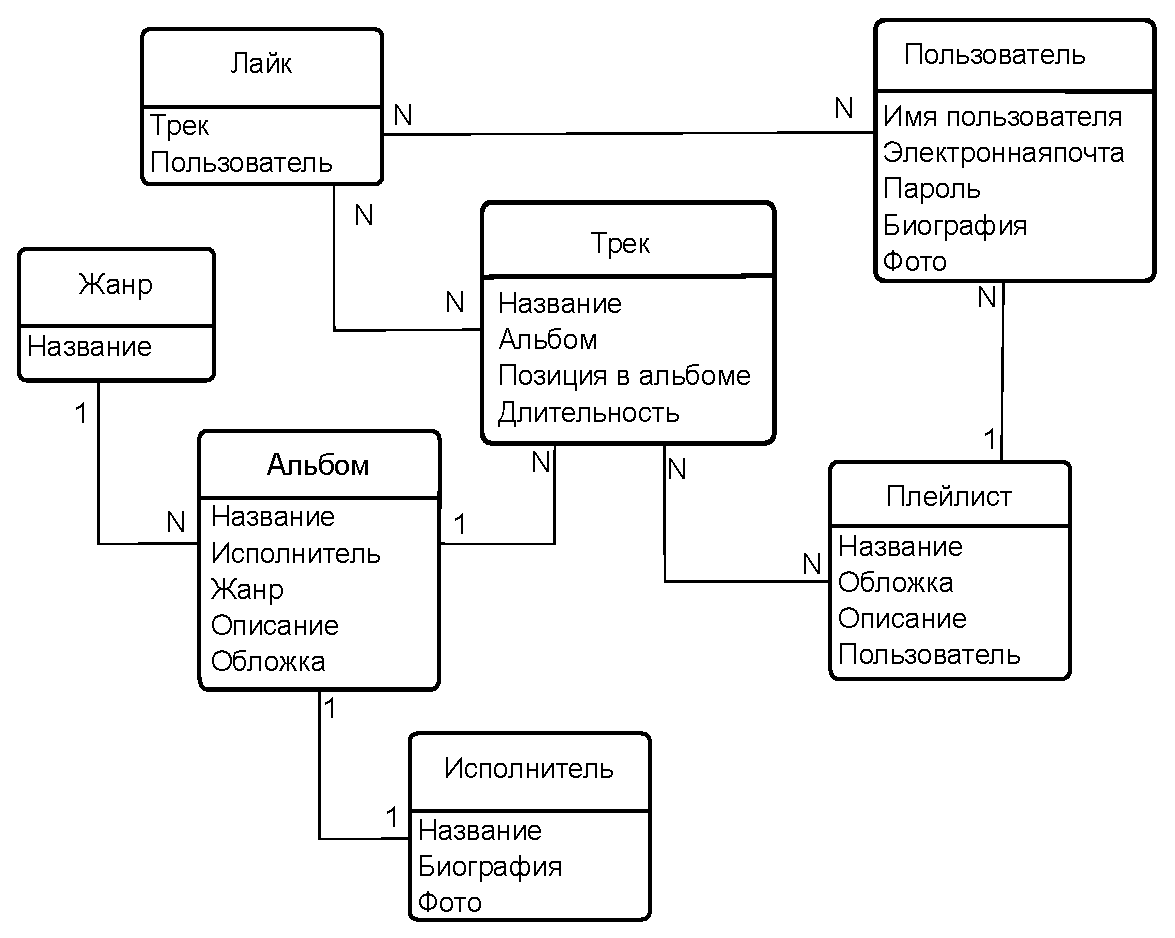
\includegraphics[width=0.7\linewidth]{conc_data}}
	\caption{Концептуальная модель данных}
	\label{concept_data:image}
\end{figure}

\subsubsection{Функиональные требования к программной системе}

К разрабатываемой системе могут получать доступ зарегистрированные и незарегистрированные пользователи. Для незарегистрированных пользователей должна быть реализована функция регистрации в системе.
Для зарегистрированных пользователей должны быть доступны следующие функции:
\begin{enumerate}
	\item Вход по электронной почте и паролю.
	\item Прослушивание выбранных треков.
	\item Поиск по музыкальному каталогу.
	\item Просмотр страниц артистов, альяомов и плейлистов.
	\item Отметка понравившихся треков.
	\item Удаление отметки с отмеченного трека.
	\item Просмотр отмеченных треков.
	\item Создание и удаление созданных пользователем плейлистов.
	\item Добавление и удаление треков из плейлистов.
\end{enumerate}

\paragraph{Моделирование вариантов использования}

Для создаваемого веб-сервиса была разработана модель, позволяющая наглядно демонстрировать различные способы использования сайта. Эта модель способствует физическому проектированию и тщательному анализу связей между элементами системы. В процессе создания диаграммы использования сайта используется стандарт UML для визуального моделирования\cite{uml2}.

Такая диаграмма отражает функциональные задачи, которые система будет выполнять в ходе своей работы, представляя первоначальное концептуальное видение системы на этапах ее проектирования и разработки. Разрабатываемая система изображается через серию сценариев взаимодействия, доступных пользователям или другим внешним агентам. Взаимодействующие с системой агенты могут быть людьми или техническими устройствами, и каждый сценарий описывает серию действий, доступных этим агентам.

После проведения анализа предметной области и функциональных требований были составлены диаграммы прецедентов для неавторизованного и авторизованного пользователей, представленные на рисунках \ref{uc_noauth:image} и \ref{uc_auth:image}
\vspace{1cm}
\begin{figure}[h]
	\center{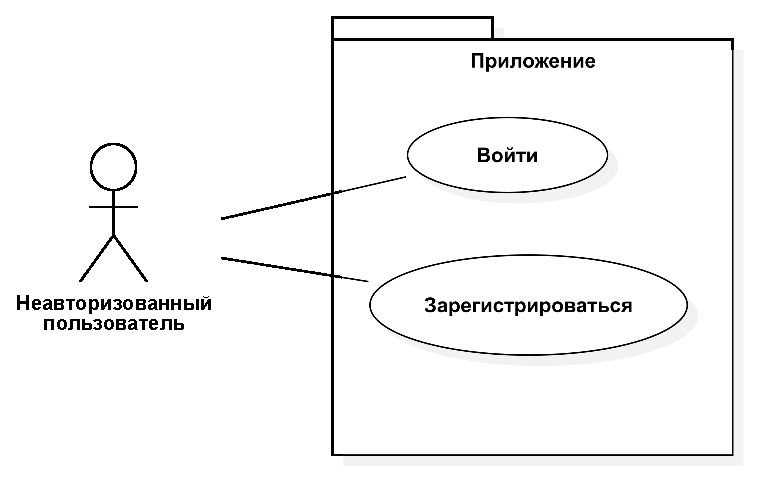
\includegraphics[width=1\linewidth]{uc_noauth}}
	\caption{Диаграмма прецедентов для неавторизованного пользователя}
	\label{uc_noauth:image}
\end{figure}

\begin{figure}[h]
	\center{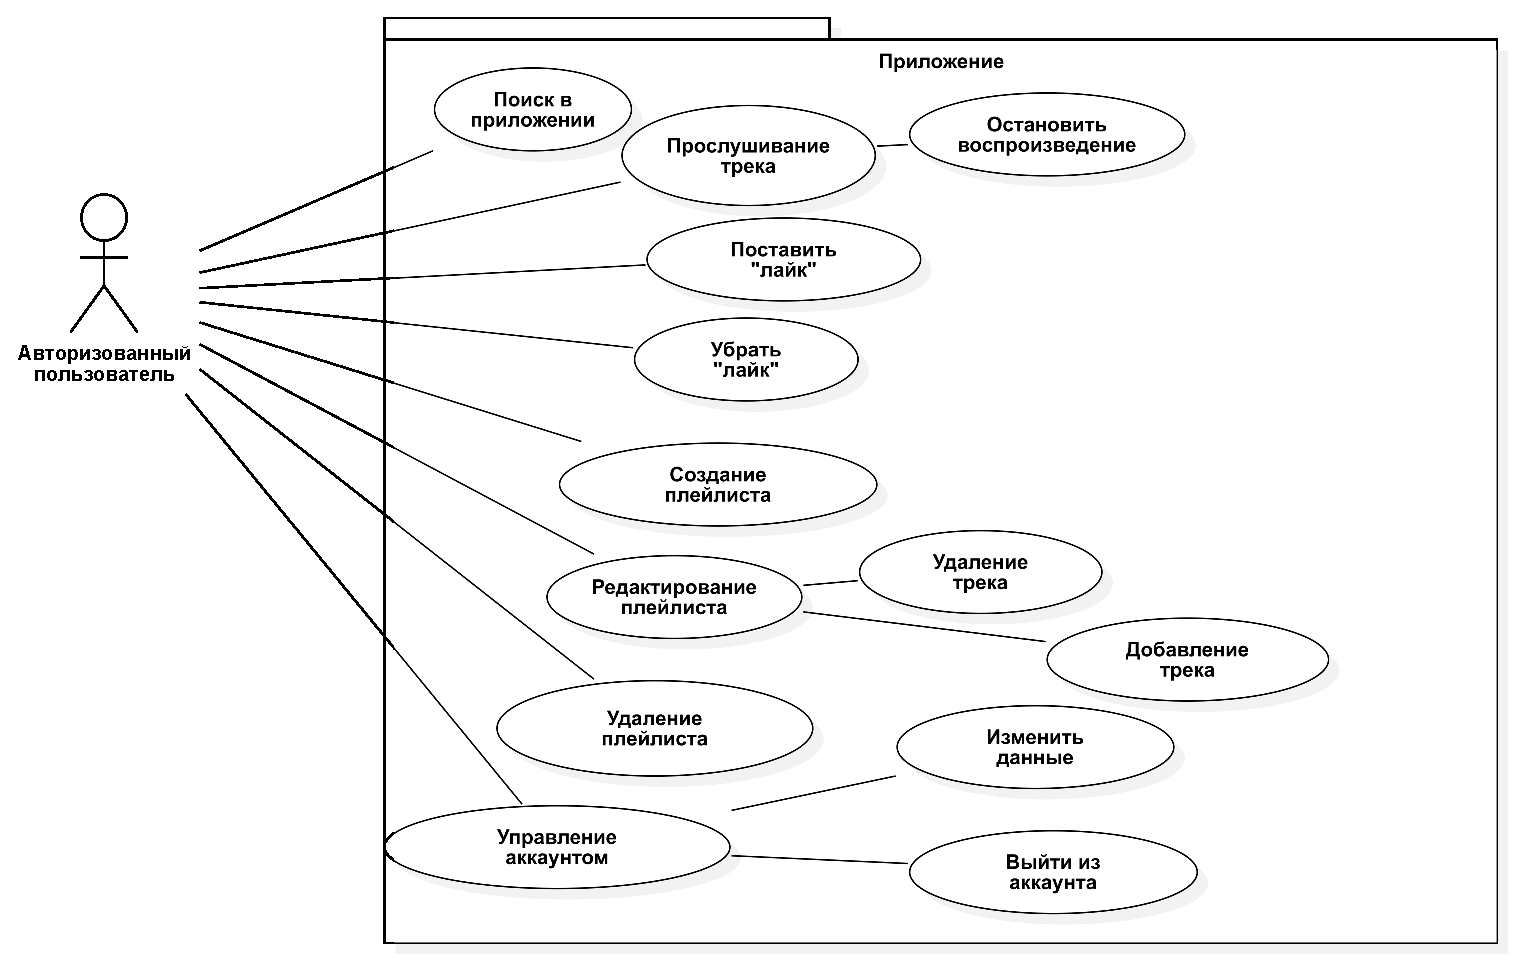
\includegraphics[width=1\linewidth]{uc_auth}}
	\caption{Диаграмма прецедентов для неавторизованного пользователя}
	\label{uc_auth:image}
\end{figure}
\paragraph{Вариант использования "<Регистрация">}

Участники
\begin{itemize}
	\item потенциальный пользователь - человек, желающий создать новую учетную запись.
\end{itemize}

Предусловия:
\begin{itemize}
	\item потенциальный пользователь имеет доступ к интернету;
	\item потенциальный пользователь посещает веб-сайт или открывает приложение, где требуется регистрация.
\end{itemize}

Постусловия:
\begin{itemize}
	\item У пользователя создана учетная запись, он может использовать свой логин и пароль для доступа к сервису;
	\item пользовательская информация сохранена в базе данных сервиса.
\end{itemize}

Основной поток событий:
\begin{enumerate}
	\item Пользователь выбирает опцию "<Регистрация"> на странице.
	\item Пользователь вводит требуемую информацию в форму регистрации: имя пользователя, адрес электронной почты и пароль.
	\item Система проверяет введенные данные на корректность и уникальность.
	\item Система подтверждает успешное создание учетной записи;
	\item Пользователю предоставляется доступ к своему профилю и основным функциям сервиса.
\end{enumerate}

Альтернативные потоки:
\begin{enumerate}
	\item Электронная почта уже используется.
	\begin{enumerate}
		\item Если введенный адрес электронной почты уже зарегистрирован в системе, пользователю предлагается войти в систему.
	\end{enumerate}
	
	\item Ошибка валидации данных.
	\begin{enumerate}
		\item Если данные не проходят валидацию, например, слабый пароль или неправильный формат электронной почты, система выводит соответствующее сообщение об ошибке, и пользователь должен исправить данные.
	\end{enumerate}
\end{enumerate}

\paragraph{Вариант использования "<Вход">}

Участники:
\begin{itemize}
	\item зарегистрированный пользователь - человек, желающий войти в свою учетную запись;
\end{itemize}

Предусловия:
\begin{itemize}
	\item зарегистрированный пользователь имеет активную учетную запись.
\end{itemize}

Постусловия:
\begin{itemize}
	\item пользователь успешно входит в систему;
	\item пользователю предоставляется доступ к своему профилю и персонализированным функциям сервиса.
\end{itemize}

Основной поток событий:
\begin{enumerate}
	\item Пользователь выбирает опцию "<Войти"> на странице.
	\item Пользователь вводит свой адрес электронной почты и пароль в форму входа.
	\item Система проверяет введенные данные на соответствие зарегистрированному профилю.
	\item Система подтверждает успешный вход в систему.
	\item Пользователю открывается доступ к интерфейсу системы.
\end{enumerate}

Альтернативные потоки:
\begin{enumerate}
	\item Неверный логин или пароль.
	\begin{enumerate}
		\item Если данные не соответствуют ни одному из профилей в системе, пользователю предлагается попробовать ввести данные снова.
	\end{enumerate}
\end{enumerate}

\paragraph{Вариант использования "<Поиск">}

Участники:
\begin{itemize}
	\item зарегистрированный пользователь.
\end{itemize}

Предусловия:
\begin{itemize}
	\item зарегистрированный пользователь имеет активную учетную запись и вошел в систему.
\end{itemize}

Постусловия:
\begin{itemize}
	\item пользователь получает результаты, совпадающие с введенной строкой поиска.
\end{itemize}

Основной поток событий:
\begin{enumerate}
	\item Пользователь вводит строку поиска в поле "<Поиск"> на странице.
	\item Система находит запрошенные данные на сервере.
	\item Пользователь получает список совпадений с введенной строкой.
\end{enumerate}

Альтернативные потоки:
\begin{enumerate}
	\item Отсутствие совпадений.
	\begin{enumerate}
		\item Если система не находит запрошенную информацию, пользователь получает сообщение об отсутствии совпадений.
	\end{enumerate}
\end{enumerate}

\paragraph{Вариант использования "<Прослушать трек">}

Участники:
\begin{itemize}
	\item зарегистрированный пользователь.
\end{itemize}

Предусловия:
\begin{itemize}
	\item зарегистрированный пользователь имеет активную учетную запись и вошел в систему.
\end{itemize}

Постусловия:
\begin{itemize}
	\item трек проигрывается через медиаплеер на устройстве пользователя.
\end{itemize}

Основной поток событий:
\begin{enumerate}
	\item Пользователь выбирает трек для прослушивания, нажимая на сам трек.
	\item Система запускает медиаплеер и начинает воспроизведение выбранного трека.
	\item Во время прослушивания пользователь может управлять воспроизведением.
\end{enumerate}

Альтернативные потоки:
\begin{enumerate}
	\item Прерывание воспроизведения.
	\begin{enumerate}
		\item Пользователь может в любой момент остановить воспроизведение трека, выбрав опцию "<Стоп">.
		\item Система останавливает воспроизведение и ждет других команд.
	\end{enumerate}
\end{enumerate}

\paragraph{Вариант использования "<Поставить "<лайк">">}

Участники:
\begin{itemize}
	\item зарегистрированный пользователь.
\end{itemize}

Предусловия:
\begin{itemize}
	\item зарегистрированный пользователь имеет активную учетную запись и вошел в систему.
\end{itemize}

Постусловия:
\begin{itemize}
	\item трек отмечается иконкой "<лайк">;
	\item система сохраняет "<лайк"> в базу данных.
\end{itemize}

Основной поток событий:
\begin{enumerate}
	\item Пользователь выбирает опцию "<Поставить "<лайк">"> у трека>.
\end{enumerate}

\paragraph{Вариант использования "<Удалить "<лайк">">}

Участники:
\begin{itemize}
	\item зарегистрированный пользователь.
\end{itemize}

Предусловия:
\begin{itemize}
	\item зарегистрированный пользователь имеет активную учетную запись и вошел в систему;
	\item трек отмечен "<лайком">".
\end{itemize}

Постусловия:
\begin{itemize}
	\item у трека удаляется иконка "<лайк">;
	\item система удаляет "<лайк"> из базы данных.
\end{itemize}

Основной поток событий:
\begin{enumerate}
	\item Пользователь выбирает опцию "<Удалить "<лайк">"> у "<лайкнутого">" трека>.
	\item Система удаляет "<лайк">.
\end{enumerate}

\paragraph{Вариант использования "<Создание плейлиста">}

Участники:
\begin{itemize}
	\item зарегистрированный пользователь.
\end{itemize}

Предусловия:
\begin{itemize}
	\item зарегистрированный пользователь имеет активную учетную запись и вошел в систему.
\end{itemize}

Постусловия:
\begin{itemize}
	\item пользователь получает созданный плейлист;
	\item система сохраняет плейлист в базу данных.
\end{itemize}

Основной поток событий:
\begin{enumerate}
	\item Пользователь выбирает опцию "<Создать плейлист">.
	\item Система отображает форму ввода данных.
	\item Пользователь вводит данные.
	\item Система сохраняет плейлист.
\end{enumerate}
	
Альтернативные потоки:
\begin{enumerate}
	\item Отмена создания.
	\begin{enumerate}
		\item Если пользователь передумал создавть плейлист, он нажимает кнопку "<Отмена">.
	\end{enumerate}
\end{enumerate}

\paragraph{Вариант использования "<Редактирование плейлиста">}


Участники:
\begin{itemize}
	\item зарегистрированный пользователь.
\end{itemize}

Предусловия:
\begin{itemize}
	\item зарегистрированный пользователь имеет активную учетную запись и вошел в систему.
\end{itemize}

Постусловия:
\begin{itemize}
	\item пользователь получает измененный плейлист;
	\item система сохраняет изменения плейлиста в базу данных.
\end{itemize}

Основной поток событий:
\begin{enumerate}
	\item Пользователь выбирает опцию "<Изменить плейлист">.
	\item Пользователь выбирает один или несколько треков, которые хочет удалить.
	\item После изменений пользователь выбирает опцию "<Сохранить изменения">.
\end{enumerate}

Альтернативные потоки:
\begin{enumerate}
	\item Отмена изменений.
	\begin{enumerate}
		\item Если пользователь решил не изменять плейлист, он выбирает опцию "<Отменить">.
	\end{enumerate}
\end{enumerate}

\paragraph{Вариант использования "<Удаление плейлиста">}

Участники:
\begin{itemize}
	\item зарегистрированный пользователь.
\end{itemize}

Предусловия:
\begin{itemize}
	\item зарегистрированный пользователь имеет активную учетную запись и вошел в систему.
\end{itemize}

Постусловия:
\begin{itemize}
	\item плейлист пропадает из списка плейлистов;
	\item система удаляет плейлист из базы данных.
\end{itemize}

Основной поток событий:
\begin{enumerate}
	\item Пользователь выбирает опцию "<Удалить плейлист">.
	\item Система просит пользователя подтвердить удаление.
	\item После подтверждения пользователя система удаляет плейлист.
\end{enumerate}

Альтернативные потоки:
\begin{enumerate}
	\item Отмена удаления.
	\begin{enumerate}
		\item Если пользователь не удалять плейлист, он выбирает опцию "<Отменить"> в диалоге подтверждения.
	\end{enumerate}
\end{enumerate}

\paragraph{Вариант использования "<Изменить профиль">}

Участники:
\begin{itemize}
	\item зарегистрированный пользователь.
\end{itemize}

Предусловия:
\begin{itemize}
	\item зарегистрированный пользователь имеет активную учетную запись и вошел в систему.
\end{itemize}

Постусловия:
\begin{itemize}
	\item профиль пользователя обновляется с новыми данными;
	\item изменения сохраняются в базе данных.
\end{itemize}

Основной поток событий:
\begin{enumerate}
	\item Пользователь выбирает опцию "<Изменить профиль">.
	\item Система предоставляет форму для ввода или изменения данных профиля.
	\item Пользователь вносит желаемые изменения в поля формы.
	\item Пользователь подтверждает изменения, выбирая опцию "<Сохранить изменения">.
	\item Система проверяет введенные данные на корректность.
	\item После проверки система обновляет информацию в профиле пользователя.
	\item Система уведомляет пользователя о успешном обновлении профиля.
\end{enumerate}

Альтернативные потоки:
\begin{enumerate}
	\item Отмена изменений.
	\begin{enumerate}
		\item Если пользователь решает не изменять профиль, он может выбрать опцию "<Отмена"> или закрыть форму изменения профиля.
		\item Система возвращает пользователя на предыдущую страницу без сохранения изменений.
	\end{enumerate}
	\item Ошибка ввода данных.
	\begin{enumerate}
		\item Если введенные данные не соответствуют требованиям (например, имя пользователя слишком длинное или содержит недопустимые символы), система выдает сообщение об ошибке.
		\item Пользователь возвращается к форме для корректировки данных.
	\end{enumerate}
\end{enumerate}

\paragraph{Вариант использования "<Выйти из профиля">}

Участники:
\begin{itemize}
	\item зарегистрированный пользователь.
\end{itemize}

Предусловия:
\begin{itemize}
	\item зарегистрированный пользователь имеет активную учетную запись и вошел в систему.
\end{itemize}

Постусловия:
\begin{itemize}
	\item пользователь выходит из своего профиля;
\end{itemize}

Основной поток событий:
\begin{enumerate}
	\item Пользователь нажимает на опцию "<Выйти"> в панели пользователя.
	\item Система перенаправляет пользователя на страницу входа.
\end{enumerate}


\subsubsection{Требования к пользовательскому интерфейсу}

Для системы дожен быть реализован пользовательский интерфейс на основе веб-технологий\cite{jshtml}\cite{ui2}. Доступ к интерфейсу осуществляется чере веб-браузер. Должна быть предусмотрена возможность адаптации под мобильные экраны.
Интерфейс должен включать в себя:
\begin{itemize}
	\item страницы для авторизации и регистрации;
	\item главная страница для авторизованного пользователя;
	\item поиск по исполнителям, альбомам, трекам, плейлистам;
	\item страница исполнителя;
	\item страница альбома;
	\item страница плейлиста;
	\item плеер для прослушивания треков;
	\item профиль пользователя.
\end{itemize}

\subsubsection{Требования к программному обеспечению}

Для реализации программной системы должны быть использованы
следующие языки программирования:
\begin{itemize}
	\item Java - серверная часть приложеня;
	\item JavaScript - клиентская часть приложения, запросы MongoDB;
	\item SQL  - для запросов в базу данных.
\end{itemize}
Для доступа к клиентской части требуется веб-браузер с поддержкой JavaScript стандарта ECMAScript 2015.

\subsection{Требования к оформлению документации}

Разработка программной документации и программного изделия должна производиться согласно ГОСТ 19.102-77 и ГОСТ 34.601-90. Единая система программной документации.
